\documentclass[10pt,letterpaper]{article}

% ---------- Encoding & fonts ----------
\usepackage[utf8]{inputenc}
\usepackage[T1]{fontenc}
\usepackage{lmodern}
\usepackage{microtype}

% ---------- Page geometry ----------
\usepackage[margin=1in]{geometry}

% ---------- Math ----------
\usepackage{amsmath, amssymb, amsthm, mathtools}
\usepackage{bm}

% ---------- Tables & figures ----------
\usepackage{booktabs}
\usepackage{tabularx}
\usepackage{multirow}
\usepackage{caption}
\captionsetup{font=small}
\usepackage[section,above]{placeins}
\usepackage{xcolor}

% ---------- TikZ ----------
\usepackage{tikz}
\usetikzlibrary{arrows.meta,positioning,fit,shapes,backgrounds,calc}
\definecolor{zirenlight}{HTML}{F2F2F2}
\definecolor{zirenslate}{HTML}{999999}

% ---------- Authors ----------
\usepackage{authblk}
\renewcommand\Authfont{\normalsize}
\renewcommand\Affilfont{\small}

% ---------- References & hyperlinks ----------
\usepackage[numbers,sort&compress]{natbib}
\usepackage{hyperref}
\hypersetup{
  colorlinks=true,
  linkcolor=black,
  citecolor=black,
  urlcolor=blue,
  pdftitle={Hash-Only Recursion for Ziren: KoalaBear--Blake3 Core Proofs and a Compiled Compress Stage over GF(2^128)},
  pdfauthor={ZKM Team},
}
\usepackage{url}

% ---------- Theorem environments ----------
\newtheorem{theorem}{Theorem}[section]
\newtheorem{lemma}[theorem]{Lemma}
\newtheorem{proposition}[theorem]{Proposition}
\theoremstyle{definition}
\newtheorem{definition}[theorem]{Definition}
\newtheorem{example}[theorem]{Example}
\theoremstyle{remark}
\newtheorem{remark}[theorem]{Remark}
\theoremstyle{plain}

% ---------- Macros ----------
\newcommand{\F}{\ensuremath{\mathbb{F}}}
\newcommand{\Fp}{\ensuremath{\mathbb{F}_{p}}}
\newcommand{\EF}{\ensuremath{\mathbb{F}_{p^4}}}
\newcommand{\Ft}{\ensuremath{\mathbb{F}_{2^{128}}}}
\newcommand{\GFtwo}{\ensuremath{\mathbb{F}_{2}}}
\newcommand{\KB}{\ensuremath{\mathsf{KoalaBear}}}
\newcommand{\WHIR}{\ensuremath{\mathsf{WHIR}}}
\newcommand{\Blake}{\ensuremath{\mathsf{Blake3}}}
\newcommand{\Poseidon}{\ensuremath{\mathsf{Poseidon2}}}
\newcommand{\LogUp}{\ensuremath{\mathsf{LogUp\text{-}GKR}}}
\newcommand{\eqf}{\ensuremath{\mathsf{eq}}}
\newcommand{\RS}{\ensuremath{\mathsf{RS}}}
\newcommand{\AND}{\ensuremath{\mathsf{AND}}}
\newcommand{\MUL}{\ensuremath{\mathsf{MUL}}}
\newcommand{\XOR}{\ensuremath{\mathsf{XOR}}}
\newcommand{\Ziren}{\textsc{Ziren}}
\newcommand{\Flock}{\textsc{Flock}}
\newcommand{\Binius}{\textsc{Binius64}}
\newcommand{\zkVM}{zkVM}
\newcommand{\Mbit}{\,\text{Mbit}}
\newcommand{\Gbit}{\,\text{Gbit}}

\title{Hash-Only Recursion for \Ziren{}: \KB{}--\Blake{} Core Proofs and a Compiled Compress Stage over $\Ft$\\[0.4em]\large Design paper}

\author[1]{Stephen Duan\thanks{Corresponding author: \texttt{stephen.d@zkm.io}}}
\affil[1]{ZKM Team}

\date{October 2026}

\begin{document}

\maketitle

\begin{abstract}
We describe the design of a two-stage proof pipeline for the \Ziren{} MIPS32 \zkVM{} in which no stage uses an algebraic hash. The \emph{core} stage keeps \Ziren{}'s existing arithmetisation over \KB{} and replaces \Poseidon{} with \Blake{} in both the Merkle commitments and the Fiat--Shamir transcript, under the same jagged \WHIR{} opening. The \emph{compress} stage aggregates the core shard proofs in a binary tree whose proofs live over $\Ft$, are committed with \Blake{} Merkle trees and are opened with \WHIR{} over $\Ft$; its verifier is therefore a Boolean circuit of \Blake{} compressions and $\Ft$ arithmetic, the shape a garbled-circuit verifier consumes.

We report measurements from a working prototype of both stages. On an Ethereum mainnet block of $1.10\times 10^8$ MIPS cycles proved on two RTX~5090 GPUs, the \Blake{} core matches the \Poseidon{} configuration cold ($16.7$\,s against $16.5$\,s) and trails it warm ($15.0$\,s against $11.5$\,s), with all of the difference in the \WHIR{} commitments; its shard proofs are $11\%$ smaller. The prototype compress stage, a multi-STARK over $\Ft$ that emulates \KB{} arithmetic bit by bit, needs $2$\,h\,$58$\,min for the same block. We trace that cost to its leaves, where an emulated \KB{} multiplication costs about two thousand \AND{} constraints and the multiplication table holds roughly two thirds of the committed bits.

The main contribution is the design of a \emph{compress compiler} that replaces the emulated machine. It lowers each recursion verifier, which is a straight-line program fixed by the shape of the proof it verifies, into a registry of uniform gate tables in the style of \Flock{}: Boolean tables in rank-one form over $\GFtwo$ for hashing and bit manipulation, $\Ft$ element tables for the native arithmetic of the tree's own verifier, and 64-bit word tables with an integer-multiplication constraint, proved in the exponent as in \Binius{}, for \KB{} arithmetic. A static copy-constraint argument replaces the memory and bus tables of the emulated machine. We state the protocol stack, compare it with \Flock{} and \Binius{}, estimate its cost from measured operation counts, and list what remains to be measured.
\end{abstract}

\noindent\textbf{Index terms:} binary fields, garbled circuits, GKR, polynomial commitment schemes, recursive proof composition, R1CS, WHIR, zero-knowledge virtual machines.

\section{Introduction}\label{sec:intro}

\Ziren{} proves MIPS32 execution in two stages. A \emph{core} stage splits an execution into shards and proves each shard with a lookup argument, a zerocheck and a jagged commitment opened through \WHIR{}~\citep{whir,jagged-pcs}; a \emph{compress} stage verifies the shard proofs recursively until one proof remains. In the deployed configuration both stages work over \KB{} and hash with \Poseidon{}~\citep{poseidon2}, an arithmetisation-friendly permutation whose cost inside a prime-field circuit is small.

This paper designs the pipeline for a different consumer: a verifier that runs as a Boolean circuit. Garbled-circuit verification~\citep{yao86,free-xor,half-gates}, as used by recent \textsc{Bitcoin} bridge designs~\citep{bitvm,bitvm3,glock}, charges for every \AND{} gate of the verifier and nothing for \XOR{}. Under that cost model an algebraic hash is the wrong choice: a \Poseidon{} permutation over a 31-bit prime expands into hundreds of thousands of Boolean constraints, while a \Blake{} compression~\citep{blake3} costs about ten thousand. Prime-field arithmetic is the wrong choice for the same reason. The verifier we want hashes with \Blake{} and computes in a binary field, where addition is \XOR{}.

\paragraph{Target.} The design fixes two choices.
\begin{enumerate}
  \item \textbf{Core: \KB{} with \Blake{}.} The core stage keeps \Ziren{}'s arithmetisation over \KB{}, unchanged, and replaces \Poseidon{} by \Blake{} in its Merkle trees and its transcript. The shard prover remains a GPU prover over a 31-bit field (\S\ref{sec:core}).
  \item \textbf{Compress: $\Ft$ with \Blake{}, in the style of \Flock{}.} Every proof of the compress tree lives over $\Ft$, commits with \Blake{} Merkle trees and opens with \WHIR{}~\citep{whir} over $\Ft$. Its circuits are produced by a compiler from the recursion verifier programs (\S\ref{sec:compiler}, \S\ref{sec:protocol}).
\end{enumerate}
Both stages therefore use one commitment family, \WHIR{} with \Blake{} Merkle trees, over two fields.

\paragraph{Where the cost is.} The leaves of the compress tree verify \KB{} proofs, so their circuits must perform \KB{} arithmetic in a field of characteristic two. A first prototype does this with a multi-STARK over $\Ft$ whose tables emulate \KB{} multiplication bit by bit. It works end to end on a real block, and it is slow: $2$\,h\,$58$\,min for a block whose core proof takes $15$\,s (\S\ref{sec:cost}). The cost is concentrated in one place. An emulated \KB{} base-field multiplication costs about $2{,}000$ \AND{} constraints and a degree-four extension multiplication $20$--$31$ thousand; extension multiplications are half of a leaf verifier's operations, and the multiplication table holds about two thirds of a leaf's committed bits.

\paragraph{Approach.} Two recent systems prove large computations over binary fields efficiently, and each solves half of our problem.
\Flock{}~\citep{flock} proves batches of identical Boolean circuits written in rank-one form over $\GFtwo$, with a zerocheck, a lincheck that exploits the batch structure, and a product-GKR wiring argument that connects heterogeneous gate tables into one circuit. It has no integer or prime-field arithmetic.
\Binius{}~\citep{binius64} proves constraint systems over 64-bit words whose only nonlinear constraints are a word-wide \AND{} and a 64-bit unsigned multiplication; the multiplication is checked in the exponent of the multiplicative group of $\Ft$ by a short GKR~\citep{gkr-cmt}.
Our compiler takes the table-and-wiring structure of \Flock{} and adds the word multiplication of \Binius{} for exactly the operations that need it.

\paragraph{Contributions.}
\begin{itemize}
  \item A measured baseline for both stages on an Ethereum mainnet block, with the core compared against the deployed \Poseidon{} configuration on the same guest program and the same two GPUs (\S\ref{sec:core-measurements}), and a decomposition of the prototype compress stage's cost (\S\ref{sec:cost-baseline}).
  \item The design of a compress compiler that lowers recursion verifier programs to three classes of uniform gate tables and a static copy-constraint argument, with explicit lowering rules for every verifier operation (\S\ref{sec:compiler}, Appendix~\ref{app:lowering}).
  \item The protocol stack that proves the compiled circuits under \WHIR{} over $\Ft$ with \Blake{} Merkle trees, and the shape of the recursion tree (\S\ref{sec:protocol}).
  \item A comparison with \Flock{} and \Binius{} (\S\ref{sec:comparison}), a cost estimate from measured operation counts (\S\ref{sec:cost}), a GPU design with measured kernels (\S\ref{sec:gpu}), and the soundness obligations the design introduces (\S\ref{sec:soundness}).
\end{itemize}

\paragraph{Status.} Everything in \S\ref{sec:core} and the baseline of \S\ref{sec:cost-baseline} is implemented and measured. The compiler, its table classes and its protocol are a design; \S\ref{sec:status} separates what is built from what is proposed and states the measurements that decide the design.

\section{Preliminaries}\label{sec:prelim}

\paragraph{Fields.} \KB{} is the prime field $\Fp$ with $p = 2^{31} - 2^{24} + 1$. The core stage draws challenges from the binomial extension $\EF = \Fp[X]/(X^4 - 3)$. A product of two canonical \KB{} representatives is below $2^{62}$, and a sum of four such products is below $2^{64}$.

$\Ft$ is the binary field of $2^{128}$ elements. Addition is bitwise \XOR{}. We use two bases: the tower basis, in which the stage's subfield structure is visible, and the polynomial basis $\GFtwo[x]/(x^{128}+x^7+x^2+x+1)$, in which a multiplication is a carry-less product followed by a reduction. The change between them is $\GFtwo$-linear. $\Ft^{*}$ is cyclic of order $2^{128}-1$; we fix a generator $g$.

\paragraph{Multilinear polynomials.} A vector $v \in \F^{2^\ell}$ is identified with its multilinear extension $\tilde v$ on $\F^\ell$. For $r \in \F^\ell$, $\eqf(r, x) = \prod_i (r_i x_i + (1-r_i)(1-x_i))$, so that $\tilde v(r) = \sum_{x \in \{0,1\}^\ell} \eqf(r,x)\,v(x)$.

\paragraph{Sumcheck, zerocheck and GKR.} The sumcheck protocol~\citep{lund1992algebraic} reduces a claim about $\sum_x f(x)$ to one evaluation of $f$. A zerocheck proves that a polynomial constraint vanishes on the Boolean hypercube by a sumcheck of the constraint against $\eqf(r,\cdot)$ at a random $r$. The GKR protocol~\citep{gkr-cmt} proves the output of a layered circuit by one sumcheck per layer; a \emph{product GKR} proves a grand product $\prod_x v(x)$ by a binary tree of multiplications.

\paragraph{Rank-one constraint systems.} An R1CS over a field $\F$ with matrices $A,B,C$ is satisfied by $z$ when $(Az)\circ(Bz) = Cz$. We use the identity-output form $C = I$, in which every constraint defines one witness entry: $(Az)_i \cdot (Bz)_i = z_i$. A \emph{batched} R1CS repeats one base block $A_0, B_0 \in \F^{k\times k}$ over $2^n$ instances, $A = I_{2^n} \otimes A_0$, so that its matrices have the description size of one block.

\paragraph{Customizable constraint systems.} CCS~\citep{ccs} writes a constraint system as $\sum_i c_i \bigcirc_{j\in S_i} M_j z = 0$. An AIR over consecutive rows is the special case with one identity matrix and one shift matrix, and introduces no auxiliary variables; R1CS is the case of three matrices and products of degree two. We use CCS only as a vocabulary: every table of the compiler is an R1CS or an AIR, and both are CCS.

\paragraph{WHIR.} \WHIR{}~\citep{whir} is a Reed--Solomon proximity test that doubles as a multilinear polynomial commitment: the prover commits a codeword with a Merkle tree, and each round folds the polynomial by a factor $2^{\kappa}$, commits the folded codeword at a lower rate, and answers queries with Merkle paths. Over $\Ft$ the code is an additive Reed--Solomon code evaluated on an $\GFtwo$-affine subspace, and encoding is an additive NTT~\citep{binius,fri-binius}.

\paragraph{Boolean cost model.} We count the cost of a verifier circuit in \AND{} gates. \XOR{} and \textsf{NOT} are free, as in free-\XOR{} garbling~\citep{free-xor}. A \Blake{} compression costs $10{,}298$ \AND{} constraints in \Flock{}'s circuit~\citep{flock} and $10{,}416$ in ours.

\section{Architecture}\label{sec:arch}

Figure~\ref{fig:pipeline} shows the pipeline. An execution of $T$ cycles is cut into shards of at most $2^{24}$ cycles. Each shard is proved by the core stage over \KB{}. The compress stage then proves, for each shard, a \emph{leaf}: a proof over $\Ft$ that the shard proof verifies. Leaves are combined pairwise by \emph{nodes}, each a proof over $\Ft$ that two child proofs verify and that their public values chain, until one \emph{root} remains. The root's verifier is the Boolean circuit that a garbled verifier evaluates.

\begin{figure}[t]
\centering
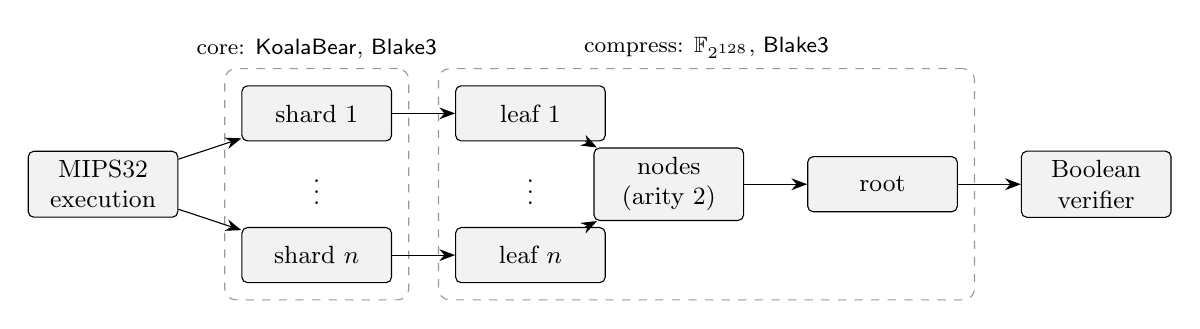
\begin{tikzpicture}[
  font=\small,
  box/.style={draw, rounded corners=2pt, minimum height=7mm, minimum width=19mm, align=center, fill=zirenlight},
  stage/.style={draw=zirenslate, dashed, rounded corners=4pt, inner sep=6pt},
  arr/.style={-{Stealth[length=2mm]}},
]
\node[box] (exec) {MIPS32\\execution};
\node[box, right=8mm of exec, yshift=9mm] (s1) {shard $1$};
\node[box, right=8mm of exec, yshift=-9mm] (sn) {shard $n$};
\node at ($(s1)!0.5!(sn)$) {$\vdots$};
\node[box, right=8mm of s1] (l1) {leaf $1$};
\node[box, right=8mm of sn] (ln) {leaf $n$};
\node at ($(l1)!0.5!(ln)$) {$\vdots$};
\node[box, right=8mm of $(l1)!0.5!(ln)$] (nodes) {nodes\\(arity 2)};
\node[box, right=8mm of nodes] (root) {root};
\node[box, right=8mm of root] (gc) {Boolean\\verifier};
\draw[arr] (exec) -- (s1); \draw[arr] (exec) -- (sn);
\draw[arr] (s1) -- (l1); \draw[arr] (sn) -- (ln);
\draw[arr] (l1) -- (nodes); \draw[arr] (ln) -- (nodes);
\draw[arr] (nodes) -- (root); \draw[arr] (root) -- (gc);
\begin{scope}[on background layer]
\node[stage, fit=(s1)(sn), label={[font=\footnotesize]above:core: $\KB$, \Blake{}}] {};
\node[stage, fit=(l1)(ln)(nodes)(root), label={[font=\footnotesize]above:compress: $\Ft$, \Blake{}}] {};
\end{scope}
\end{tikzpicture}
\caption{The two stages. Every proof is committed with \Blake{} Merkle trees and opened with \WHIR{}; the core stage works over \KB{}, the compress stage over $\Ft$.}
\label{fig:pipeline}
\end{figure}

\paragraph{Statements.} A core shard proof attests that a shard's trace satisfies the core machine's AIR and buses for a committed program, and exposes the shard's public values: the program counter pair at entry and exit, the shard index, the memory digest contribution and the committed output. A leaf attests that a core shard proof verifies against a verifying key from an enumerated allowlist and exposes the same public values. A node attests that its two children verify and that the exit state of the left child is the entry state of the right child. The root's public values are those of the whole execution.

\paragraph{Why a tree and not a chain.} Leaves are independent and can be proved in parallel, on any number of devices, as soon as their shard proofs exist. A tree of arity two over $n$ leaves has depth $\lceil \log_2 n \rceil$; in the measured block $n = 34$ (\S\ref{sec:cost-baseline}).

\paragraph{Fields across the boundary.} The leaf is the only place where the two fields meet. Its circuit verifies a \KB{} proof and must therefore perform \KB{} and $\EF$ arithmetic, \Blake{} compressions over the proof's Merkle paths, and the transcript's conversion of \Blake{} digests into \KB{} challenges. A node verifies $\Ft$ proofs, so its arithmetic is native. The design of \S\ref{sec:compiler} exists to make the leaf cheap; the node's cost follows from \Flock{}'s existing techniques.

\section{The core stage: \KB{} with \Blake{}}\label{sec:core}

The core stage keeps \Ziren{}'s arithmetisation as it is: the per-opcode instruction-frame chips, the byte and range tables, the memory argument, the shard-level \LogUp{}~\citep{logup-gkr} and zerocheck, and the jagged commitment~\citep{jagged-pcs} opened through batched \WHIR{}. Its 56 instruction and precompile chips read only their own row; no constraint refers to the next row, and the maximum constraint degree is three. None of this changes. Only the commitment's hash and the transcript change.

\subsection{The \Blake{} ring}

\paragraph{Commitments.} Traces are committed with Merkle trees whose leaves hash the canonical little-endian encodings of \KB{} elements with \Blake{}, and whose internal nodes compress two 32-byte children with \Blake{}. The \WHIR{} round commitments use the same trees.

\paragraph{Transcript.} The Fiat--Shamir transcript~\citep{fiat-shamir,bcs16} is a \Blake{} sponge-like construction that buffers observed bytes up to one block and folds them into a 32-byte state; challenges are squeezed as \KB{} elements from the state. A commitment root is observed as eight field elements, the low $30$ bits of each little-endian 32-bit word of the digest. Thirty bits lie below $p$, so the map is injective on what it keeps, and the transcript binds $240$ of the root's $256$ bits.

\paragraph{What the compress stage inherits.} The leaf verifies exactly this ring. It recomputes every Merkle path with \Blake{}, replays the transcript with \Blake{}, and slices digests into 30-bit limbs. In the Boolean cost model these are cheap: slicing is wiring, and each compression costs about $10^4$ \AND{} constraints instead of the several hundred thousand a \Poseidon{} permutation would cost.

\subsection{Measurements}\label{sec:core-measurements}

We proved Ethereum mainnet block $26{,}206{,}588$ with the same guest program under both rings: $109{,}781{,}075$ MIPS cycles in $34$ shards. Both rings ran on two RTX~5090 GPUs of the same machine with the same prover settings, in back-to-back jobs. ``Cold'' is the first block after the prover starts; ``warm'' is a second proof of the same block in the same process. For the \Poseidon{} ring the time is to a compressed proof, with recursion overlapped on the same cards, and the core phase is reported separately; for the \Blake{} ring it is the core phase alone.

\begin{table}[t]
\centering\small
\caption{Core stage, block $26{,}206{,}588$ ($1.10\times 10^8$ cycles, $34$ shards), two RTX~5090 GPUs.}
\label{tab:core}
\begin{tabular}{lrr}
\toprule
 & \Blake{} ring & \Poseidon{} ring \\
\midrule
core phase, cold & $16.7$--$17.3$\,s & $16.5$\,s \\
core phase, warm & $15.0$\,s ($7.3$\,MHz) & $11.5$\,s ($9.5$\,MHz) \\
compressed proof, warm & --- & $11.6$\,s \\
shard proofs, total & $60.5$\,MB & $68.0$\,MB \\
\bottomrule
\end{tabular}
\end{table}

\begin{table}[t]
\centering\small
\caption{Warm core phase per card, in milliseconds (the two cards are listed separately). ``Opening commits'' are the \WHIR{} round commitments made while opening.}
\label{tab:core-phases}
\begin{tabular}{lrr}
\toprule
 & \Blake{} ring & \Poseidon{} ring \\
\midrule
trace commitment & $1{,}355$ / $1{,}692$ & $102$ / $135$ \\
opening commits & $7{,}156$ / $6{,}377$ & $513$ / $436$ \\
GKR, zerocheck and evaluation claims & $5{,}404$ / $5{,}378$ & $5{,}003$ / $6{,}200$ \\
idle & $209$ / $552$ & $3{,}780$ / $3{,}503$ \\
\bottomrule
\end{tabular}
\end{table}

Table~\ref{tab:core} gives the totals and Table~\ref{tab:core-phases} the warm phase breakdown. Cold, the two rings are level. Warm, the \Blake{} ring is $30\%$ slower, and Table~\ref{tab:core-phases} places the whole difference in the \WHIR{} commitments: about $8.5$\,s per card against $0.6$\,s. The constraint work (GKR, zerocheck, evaluation claims) costs the same in both rings. The \Poseidon{} cards are idle for about $3.5$\,s per block, so the \Blake{} ring's commitment cost is partly hidden in the totals.

We have not yet split the \Blake{} ring's commitment time into encoding, hashing and data movement; the \Poseidon{} ring's kernels have been tuned over many releases and the \Blake{} ring's have not, which we expect to account for much of the gap. A 512\,MiB allocation in the \WHIR{} opening also fails on the last, largest precompile shards and is retried within the shard. Both effects are engineering rather than protocol: the two rings run the same protocol and differ only in the hash.

\section{The compress compiler}\label{sec:compiler}

The compiler turns a recursion verifier into a circuit that the compress stage proves. Its input is a straight-line program; its output is a \emph{registry} of uniform gate tables, a \emph{wiring} that connects their cells, and a \emph{layout} of the committed witness. This section describes the three; \S\ref{sec:protocol} describes how the result is proved.

\subsection{Why compile}

The prototype compress stage proves the verifier by \emph{executing} it: its multi-STARK has an instruction ledger, memory tables for constants and variables, and one table per operation family, connected by buses. That design is general, but it pays twice for generality. The ledger and memory tables hold every read and write of the program ($2^{22}$ and $2^{19}$ rows in a measured leaf) only to establish a dataflow that is known before proving. And every \KB{} multiplication goes through a table that emulates it bit by bit.

A recursion verifier needs neither kind of generality. For a fixed proof shape, the verifier is a fixed straight-line program: the same operations on the same operands in the same order, with only the values changing. The verifying keys of the core stage are enumerated in an allowlist, so the set of leaf programs is finite and known at key generation, and so is the set of node programs. A fixed program can be compiled to a fixed circuit once per shape, and its dataflow becomes a fixed permutation of cells instead of a memory argument.

\subsection{Front end: verifier programs}

\paragraph{Leaf programs.} The recursion compiler already turns the core verifier into a straight-line program over \KB{}, $\EF$, bits and \Blake{} compressions: $0.88$--$2.47$ million instructions per program in a measured block, $1.18$--$1.25$ million for a typical leaf (\S\ref{sec:cost}). The compress compiler takes this program as its input. Its operations are: \KB{} and $\EF$ addition, subtraction, multiplication and inversion; conversion between an $\EF$ element and its four \KB{} coordinates; bit decomposition of a \KB{} element; selection by a bit; equality assertion; \Blake{} compression; and the transcript's conversion of digests to \KB{} limbs.

\paragraph{Node programs.} A node verifies proofs of the compress stage itself, so its verifier works in $\Ft$. Instead of writing that verifier twice, the node program is recorded by running the stage's own verifier over a value type that records every operation applied to it. The recording agrees with the verifier on every transcript step by construction. Its operations are $\Ft$ addition (free), $\Ft$ multiplication, \Blake{} compression, bit slicing of digests, and equality assertion. A measured second-level node program has $7.1\times 10^5$ operations, of which $2.4\times 10^5$ are multiplications and $3.2\times 10^5$ additions, and hashes $1.25$\,MB in $19{,}857$ compressions.

\subsection{Middle: three table classes}

Each operation of a program is assigned to one row of one \emph{gate table}. Every row of a table is the same small circuit; a table with $m$ rows is a batch of $m$ identical blocks, which is what makes it cheap to prove (\S\ref{sec:protocol-tables}). The compiler uses three classes, chosen by what the operation computes.

\paragraph{Boolean tables (rank one over $\GFtwo$).} A Boolean table's block is an R1CS over $\GFtwo$ in identity-output form: each committed bit $z_i$ is defined by $(A_0 z)_i \cdot (B_0 z)_i = z_i$, where $A_0 z$ and $B_0 z$ are \XOR{}s of bits. \XOR{}s are substituted into the matrices and never committed; only inputs, outputs and \AND{} products are. This is \Flock{}'s circuit form~\citep{flock}. The compiler uses Boolean tables for \Blake{} compressions, for bit decompositions and slicing, for selection and for the parity checks of \S\ref{sec:compiler-words}. A \Blake{} compression block is \Flock{}'s, about $10^4$ \AND{} constraints with fused carry-save adders for the 32-bit additions.

\paragraph{Element tables (rank one over $\Ft$).} An element table's block is an R1CS whose variables are whole $\Ft$ elements: $(A_0 z_j + a)\cdot(B_0 z_j + b) = z_j$ with sparse $A_0, B_0$ over $\Ft$ and constants with disjoint supports, so that an all-zero row is satisfying. One $\Ft$ multiplication is one constraint, where a Boolean table would need about $2{,}187$. The compiler uses element tables for the arithmetic of node programs. This is \Flock{}'s large-field table class.

\paragraph{Word tables (64-bit \AND{} and \MUL{}).}\label{sec:compiler-words} A word table's variables are 64-bit words, and its constraints are of two kinds, as in \Binius{}~\citep{binius64}:
\[
\textstyle \AND:\ \big(\bigoplus_i w_{a_i} \ll s_i\big) \mathbin{\&} \big(\bigoplus_j w_{b_j} \ll t_j\big) = \bigoplus_k w_{c_k} \ll u_k,
\qquad
\MUL:\ p \cdot q = 2^{64}\,h + \ell,
\]
where each operand of a \MUL{} is likewise an \XOR{} of shifted words and the product is over the integers. Shifts and \XOR{}s are free. A 64-bit integer addition costs one \AND{} constraint on its carry word. The compiler uses word tables for all \KB{} and $\EF$ arithmetic.

\subsection{Lowering \KB{} arithmetic}

A \KB{} element is held as a word whose value is its canonical representative, below $p$. Every word that holds a \KB{} element is range-checked once, where it is produced; consumers rely on the wiring. With $\delta = 2^{64} - p$, the check $c < p$ is the absence of a carry in $c + \delta$, one \AND{} constraint.

\paragraph{Multiplication.} To prove $c = a\cdot b \bmod p$ the prover supplies the quotient $k$ and the circuit checks
\[
a \cdot b = 2^{64}\cdot 0 + \ell, \qquad k \cdot p = 2^{64}\cdot 0 + \ell', \qquad \ell' + c = \ell, \qquad c < p .
\]
That is two \MUL{} constraints, one addition and one range check: two \MUL{}s and two \AND{}s. Both products are below $2^{62}$, so both high words are the constant zero.

\paragraph{Extension multiplication.} For $x, y \in \EF$ with coordinates $x_i, y_j$, each output coordinate is $\sum_{i+j=t} x_i y_j + 3\sum_{i+j=t+4} x_i y_j$, a sum of four products. The circuit forms the sixteen products with \MUL{}s, multiplies the wrapped ones by three with a shift and an addition, accumulates each coordinate in two words (the sum is below $2^{66}$), and reduces each coordinate once with a \MUL{} against $p$ whose high word is now live. The total is twenty \MUL{}s and about thirty \AND{}s; Karatsuba's identity lowers the product count to nine at the price of signed intermediate sums, for thirteen \MUL{}s.

\paragraph{Other operations.} Addition is one addition and one conditional subtraction of $p$, two \AND{}s. Inversion is a supplied inverse and a multiplication checked against one. Conversion between $\EF$ and its coordinates is wiring. Bit decomposition is free in a word, because a word's bits are its committed columns; it needs one \AND{} to show that the bits above $30$ are zero. Appendix~\ref{app:lowering} lists every operation with its class and cost.

\subsection{Back end: wiring and layout}\label{sec:compiler-wiring}

\paragraph{Cells and wires.} A \emph{cell} is one wireable committed value of one row of one table: an input or output port of a gate. The program's dataflow is a set of \emph{wires}, each the set of cells that must hold the same value: the producer of a value and every consumer. A wire's cells form one orbit of a permutation $\sigma$ on the cell space, and $\sigma$ is fixed by the program. Public inputs and outputs are cells of a public table whose values the verifier supplies.

\paragraph{No memory.} The prototype's ledger and memory tables disappear. A read of a constant becomes a cell of the public table or a constant in a gate's matrix; a read of a variable becomes membership of the consumer's cell in the producer's wire. There is no address, no timestamp and no multiset of reads and writes.

\paragraph{Cross-class wires.} A wire may cross table classes: a \KB{} product computed in a word table feeds a bit decomposition in a Boolean table, and a \Blake{} digest computed in a Boolean table feeds a transcript limb in a word table. The cell space is defined over \emph{words of the committed polynomial}, so that a 64-bit word, 64 packed bits and the low half of an $\Ft$ element are all comparable. The compiler places such ports at a common width and pads the rest with zeros.

\paragraph{Layout.} Each table's witness is laid out batch-major, with the row index in the low bits, and the tables are stacked into one jagged commitment~\citep{jagged-pcs} so that each table pays for its real height. The registry, the heights, the layout and a commitment to $\sigma$ together form the circuit's verifying key.

\section{Proving a compiled circuit}\label{sec:protocol}

A compiled circuit is proved by one argument per table class, one argument for the wiring, and one batched \WHIR{} opening that discharges every evaluation claim. All arguments run over $\Ft$ under one \Blake{} transcript.

\subsection{Commitment}

The prover commits once. Bits of Boolean tables, words of word tables and elements of element tables are packed into $\Ft$ elements, $128$ bits per element, and the packed columns of all tables are stacked into one jagged polynomial. Claims about individual bits are reduced to claims about packed elements by ring switching~\citep{fri-binius}, which \Flock{} merges with the jagged commitment so that its cost is proportional to the number of committed words rather than to a padded rectangle. The packed polynomial is encoded with an additive Reed--Solomon code over an $\GFtwo$-affine subspace of $\Ft$ and committed with a \Blake{} Merkle tree.

\paragraph{Opening.} Every argument below ends in evaluation claims on the committed polynomial. They are batched by random linear combination into one claim and opened with \WHIR{} over $\Ft$. In the prototype's configuration the first codeword has rate $1/8$ and each \WHIR{} round folds by $2^4$ while lowering the rate by $2^3$. Merkle leaves are rows of $\Ft$ elements hashed with \Blake{}.

\subsection{Gate tables}\label{sec:protocol-tables}

\paragraph{Boolean and element tables.} For a table with base block $(A_0, B_0)$ and $2^n$ rows, the prover shows $(A z)\circ(B z) = z$ with $A = I_{2^n}\otimes A_0$. Following \Flock{}, a zerocheck reduces the constraint to claims on $\widetilde{Az}$, $\widetilde{Bz}$ and $\tilde z$ at one point, and a \emph{lincheck} reduces the claims on $\widetilde{Az}$ and $\widetilde{Bz}$ to claims on $\tilde z$. The lincheck exploits the block structure: the prover sends one vector of length $k$ (the block width) and the verifier checks two bilinear forms against $A_0$ and $B_0$, at a cost proportional to their number of nonzeros and independent of $n$. As in \Flock{}, the first rounds of the zerocheck use a univariate skip over a small subspace, so that the prover's first, most expensive rounds work on short univariate polynomials instead of multilinear halvings.

\paragraph{Matrix evaluations.} The verifier's bilinear forms read the base blocks. For a \Blake{} block they have about $2\times 10^7$ nonzeros, most of \Flock{}'s verification time. A recursion verifier cannot afford that work in its circuit. \Flock{} defers the matrix work as claims and folds it across levels. We instead commit the multilinear extensions of each table's base matrices once, as preprocessed polynomials of the registry, and open them in the same batched \WHIR{} opening; the verifier's matrix work then becomes one opening shared by every table. Which of the two is cheaper inside our node circuit is one of the open measurements of \S\ref{sec:status}.

\paragraph{Word tables.} \AND{} constraints are proved by a zerocheck over the bit columns of their operands, as for a Boolean table whose block is one constraint replicated over 64 bit positions. Shifts are handled by a \emph{shift reduction}, a sumcheck that turns claims on shifted words into claims on the committed words~\citep{binius64}.
\MUL{} constraints are proved in the exponent of $\Ft^{*}$, as in \Binius{}. For each row,
\[
\big(g^{p}\big)^{q} \;=\; \big(g^{2^{64}}\big)^{h}\cdot g^{\ell}
\]
is equivalent to $p q \equiv 2^{64} h + \ell \pmod{2^{128}-1}$. A power with a 64-bit exponent $z$ is the product $\prod_{i<64} (V^{2^i})^{z_i}$, each factor either $1$ or $V^{2^i}$ according to bit $z_i$; a product GKR of height six evaluates it, and a final sumcheck using the Frobenius map batches the 64 leaf claims into one claim on the base and one claim on the 64 bit columns of the exponent. Because our exponents are committed bit columns, those claims land directly on the committed polynomial.

\paragraph{Wraparound.} Over the integers $p q \le (2^{64}-1)^2 < 2^{128}-1$, so the left side never wraps. The right side reaches $2^{128}-1$ only when $h = \ell = 2^{64}-1$; there the prover could set $p = 0$. \Binius{} closes this case with a parity check on the least significant bits, $p_0 \wedge q_0 = \ell_0$, which costs a few \AND{} constraints per row. Our \KB{} rows never come near the boundary ($h \le 3$ in every row), but the parity check is kept so that the table's soundness does not depend on how it is used.

\subsection{Wiring}

The wiring argument proves that every wire's cells hold one value: that the committed cell values $w$ satisfy the multiset identity
\[
\{\,(w_x,\ x)\,\} \;=\; \{\,(w_x,\ \sigma(x))\,\}
\]
over the cell space. For random $\alpha,\beta$ this is the grand-product equality $\prod_x(\alpha + w_x + \beta x) = \prod_x(\alpha + w_x + \beta\sigma(x))$, proved by a product GKR with no committed intermediate oracle. It ends in claims on the cell values, which are gathered from the tables' committed words, and on $\tilde\sigma$, which is a preprocessed polynomial of the verifying key. Both go into the batched opening.

\paragraph{Characteristic two.} A logarithmic-derivative lookup argument sums fractions and needs the field's characteristic to exceed the multiplicities involved; in characteristic two it fails. The design uses no lookups. Range checks are \AND{} constraints, the dataflow is a permutation, and the only multiset argument is the grand product above, which is sound in any field.

\subsection{The recursion tree}

\paragraph{Leaves.} A leaf compiles the core verifier for one shard shape: \KB{} and $\EF$ arithmetic in word tables, \Blake{} in Boolean tables, the transcript's digest slicing in Boolean tables, and the wiring that ties them together. Its public table holds the shard's public values and the verifying-key digest that the allowlist check compares.

\paragraph{Nodes.} A node compiles the compress stage's own verifier, twice, plus the chaining of public values. Its arithmetic is $\Ft$ arithmetic in element tables, and its hashing is \Blake{} in Boolean tables. The node's statement does not depend on the leaves' shapes, only on the registry of the level below; in a tree whose levels share a registry, node programs repeat, and one compiled node circuit serves a level.

\paragraph{Root.} The root is the last node. Its verifier, the program that a garbled verifier evaluates, consists of \Blake{} compressions over the root proof's Merkle paths and transcript, and the $\Ft$ arithmetic of its sumchecks, lincheck and \WHIR{} queries. Section~\ref{sec:cost} estimates its size.

\section{Comparison with \Flock{} and \Binius{}}\label{sec:comparison}

Both systems prove large computations over binary fields, and the compiler borrows from each. This section states what is borrowed, what differs, and why. Table~\ref{tab:comparison} summarises. Our descriptions of \Flock{} are taken from its paper~\citep{flock} and its source code; those of \Binius{} from its architecture notes and protocol blueprint~\citep{binius64}.

\begin{table}[t]
\centering\small
\caption{\Flock{}, \Binius{} and the compress compiler.}
\label{tab:comparison}
\begin{tabularx}{\linewidth}{>{\raggedright\arraybackslash}p{2.6cm}XXX}
\toprule
 & \Flock{} & \Binius{} & this design \\
\midrule
statement & batches of one Boolean circuit (hash compressions), plus heterogeneous tables joined by wiring & one constraint system over 64-bit words & a fixed verifier program per proof shape \\
witness & bits; $\Ft$ elements in large-field tables & 64-bit words & bits, 64-bit words and $\Ft$ elements, by table \\
nonlinear constraints & \AND{} over $\GFtwo$; $\Ft$ product in element tables & word \AND{}; 64-bit integer \MUL{} & all three \\
integer / prime-field arithmetic & none & 64-bit \MUL{} & \KB{} and $\EF$ lowered to \MUL{} \\
lincheck & block-diagonal, cost of one block & none (constraints reference shifted words) & block-diagonal per table \\
cross-table dataflow & copy constraints by product GKR & within one system & copy constraints by product GKR \\
lookups and buses & declared in the circuit language, not proved & none & none; range checks by \AND{} \\
polynomial commitment & Ligerito over $\Ft$, $\F_{2^{256}}$ folding challenges & ring-switched, over a binary tower & \WHIR{} over $\Ft$ \\
Merkle hash, transcript & \Blake{} or SHA-256 & --- & \Blake{} \\
recursion & tower verifying its own proofs & --- & tree; leaves verify \KB{} proofs \\
\bottomrule
\end{tabularx}
\end{table}

\subsection{\Flock{}}

\paragraph{What is borrowed.} The circuit form (rank-one over $\GFtwo$ with identity output, \XOR{} substituted into the matrices), the batching of identical blocks with a lincheck whose cost is that of one block, the large-field table class, the registry of heterogeneous tables, the product-GKR wiring argument without a committed oracle, the jagged packing merged with ring switching, and the identity-padded dead rows that keep padding satisfying.

\paragraph{The statement is a program, not a batch.} \Flock{}'s headline workloads are batches of one hash function: $2^{18}$ \Blake{} compressions are one block repeated $2^{18}$ times. A recursion verifier is a single, heterogeneous computation. The compiler recovers \Flock{}'s structure by \emph{transposing} the program: each operation type becomes a table whose rows are identical, and the program's heterogeneity moves into the wiring permutation. This is how \Flock{}'s own recursion tower and its multi-table circuits are built; the difference is that our programs are produced from an existing verifier rather than written in a circuit language.

\paragraph{Prime-field arithmetic.} \Flock{} never verifies a proof over a prime field: its recursion tower verifies \Flock{} proofs, whose arithmetic is native. Our leaves must verify \KB{} proofs. In \Flock{}'s classes that arithmetic would be Boolean emulation, about $2{,}000$ \AND{} constraints per base-field multiplication, which is exactly the cost of our prototype. The word tables are the addition that \Flock{} does not have.

\paragraph{Commitment.} \Flock{} commits with Ligerito, a recursive multilinear commitment, with folding challenges in $\F_{2^{256}}$ for its 128-bit profile. We use \WHIR{} over $\Ft$ in both stages, so that the core and compress stages share one opening protocol and one proximity-gap analysis~\citep{proximity-gaps,proximity-gaps-2025}. Whether $\Ft$ challenges reach the soundness target or an extension is needed for some rounds is a parameter question (\S\ref{sec:soundness}).

\paragraph{Lookups.} \Flock{}'s circuit language lets a chip declare interactions with a channel, a message, a multiplicity and a selector, but no prover in its repository consumes them; its virtual-machine pilot checks one chip's rows and nothing across chips. We do not need them: a fixed program has a fixed dataflow, which the wiring argument covers.

\subsection{\Binius{}}

\paragraph{What is borrowed.} The \MUL{} constraint $p\cdot q = 2^{64}h + \ell$ and its proof in the exponent of $\Ft^{*}$ by a product GKR of height six, the parity check that closes the wraparound case, the treatment of shifts and \XOR{}s as free operand formers, and the shift reduction that moves claims on shifted words to the committed words.

\paragraph{Everything is not a word.} \Binius{} expresses every computation in 64-bit words. Hashes are then word circuits, and \Flock{} reports SHA-256 proving more than nine times faster than \Binius{}~\citep{flock}; bit-level circuits with carry-save adders suit hashes better. We use words only where integer multiplication is needed and keep hashes in Boolean tables.

\paragraph{No batch structure.} \Binius{} has one global constraint system and no notion of a repeated block. Our word tables are uniform per table, which gives them the same lincheck and layout as the other classes and lets the wiring argument join them.

\paragraph{Recursion and arithmetic of the verifier.} The \Binius{} documentation we consulted does not describe recursion. In our design the verifier of every compress-stage proof, including the \MUL{} GKR's, is native $\Ft$ arithmetic plus \Blake{}, so it compiles into element and Boolean tables at the next level.

\subsection{Differences from the prototype}

The prototype compress stage is an AIR-based multi-STARK over $\Ft$ that executes the verifier program. Compared with it, the compiler removes the instruction ledger and the memory tables (\S\ref{sec:compiler-wiring}), replaces the bit-emulated \KB{} multiplication table by word \MUL{} constraints, and replaces the logarithmic-derivative buses, which need care in characteristic two, by one grand-product wiring argument.

\section{Cost}\label{sec:cost}

\subsection{Measured baseline}\label{sec:cost-baseline}

We proved block $26{,}206{,}588$ end to end with the prototype: the \Blake{} core on two RTX~5090 GPUs, then the compress tree of $34$ leaves, $17$ first-level nodes and $20$ upper nodes in one process. The compress stage ran on $48$ CPU threads, with the Reed--Solomon encoding of its commitments on one GPU (\S\ref{sec:gpu}). The final proof verified. Table~\ref{tab:baseline} gives the times.

\begin{table}[t]
\centering\small
\caption{Prototype compress stage on block $26{,}206{,}588$.}
\label{tab:baseline}
\begin{tabular}{lrrr}
\toprule
stage & proofs & time each & total \\
\midrule
leaves & $34$ & $90$--$190$\,s ($442$\,s for the largest) & $70$\,min \\
first-level nodes & $17$ & $230$--$350$\,s & $74$\,min \\
upper nodes & $20$ & $90$--$120$\,s & $34$\,min \\
\midrule
compress stage & & & $2$\,h\,$58$\,min \\
\bottomrule
\end{tabular}
\end{table}

With the encoding on the CPU the same stage took $3$\,h\,$14$\,min in an earlier run, under different background load, so moving the encoding saved about $8\%$. Leaves are proved one after another, grouped by program so that one program's proving key is resident at a time; peak memory was $137$--$180$\,GB, against $426$\,GB when leaves of different programs were interleaved.

\paragraph{Where a leaf's cost is.} A leaf program has $1.18$--$1.25$ million instructions and commits $6.5$--$7.4$\,Gbit, padded to $2^{33}$. The two tallest tables are the instruction ledger and the \KB{} multiplication table, $2^{22}$ rows each. A multiplication row is $1{,}109$ bits, so the multiplication table alone commits about $4.6$\Gbit{}, roughly two thirds of the leaf.

\subsection{Operation counts}

The leaf programs' operation mix was measured on the \Poseidon{} configuration's recursion programs for a mainnet block, whose field arithmetic is that of our leaves and whose hashing differs; Table~\ref{tab:opmix} gives the median leaf. Extension multiplications are half of all operations. In a Boolean circuit the costs are about $2{,}000$ \AND{} constraints for a \KB{} multiplication, $20$--$31$ thousand for an $\EF$ multiplication and $320$ for an $\EF$ addition. Under that model a leaf costs $1.7$--$2.5\times 10^{10}$ \AND{} constraints: $65\%$ in extension multiplications, $31\%$ in the products of the prefix-sum checks, and $2\%$ in hashing.

\begin{table}[t]
\centering\small
\caption{Operations of the median leaf program.}
\label{tab:opmix}
\begin{tabular}{lr}
\toprule
operation & count \\
\midrule
$\EF$ multiplication & $528{,}511$ \\
$\EF$ addition and subtraction & $510{,}196$ \\
$\EF$ division & $4{,}702$ \\
\KB{} multiplication and division & $86{,}806$ \\
\KB{} addition and subtraction & $66{,}795$ \\
selection & $82{,}456$ \\
bit decomposition & $103{,}205$ \\
\bottomrule
\end{tabular}
\end{table}

\subsection{Estimate for the compiled leaf}

Under the lowering of \S\ref{sec:compiler}, an $\EF$ multiplication becomes twenty \MUL{} constraints and about thirty \AND{} constraints and commits about $52$ words: sixteen products, four accumulators of two words, four quotients, four reduction products of two words, the four reduced coordinates and about twelve carry words. That is about $3{,}300$ bits, against about $7{,}800$ in the prototype, where an extension multiplication occupies about seven rows of $1{,}109$ bits. The larger change is in the constraint work: the prototype's zerocheck runs over the $20$--$31$ thousand \AND{}s per multiplication, while the compiled circuit runs twenty instances of a height-six product GKR and a zerocheck over thirty word \AND{}s.

Table~\ref{tab:leaf-estimate} applies the per-operation costs to the median leaf. The hashing line uses the cost model's $2\%$ share, $32$--$49$ thousand compressions, at $2^{14}$ committed bits each. The estimate is about $2.7$\Gbit{} of committed witness against $6.5$--$7.4$\Gbit{}, with no ledger or memory tables. It is a projection from operation counts, not a measurement.

\begin{table}[t]
\centering\small
\caption{Committed bits of the median leaf, compiled (estimate).}
\label{tab:leaf-estimate}
\begin{tabular}{lrrr}
\toprule
operation & count & bits each & total \\
\midrule
$\EF$ multiplication & $528{,}511$ & $\approx 3{,}300$ & $1.76$\Gbit \\
$\EF$ addition and subtraction & $510{,}196$ & $512$ & $0.26$\Gbit \\
\KB{} multiplication & $86{,}806$ & $320$ & $0.03$\Gbit \\
\Blake{} compression & $32$--$49$k & $16{,}384$ & $0.5$--$0.8$\Gbit \\
selection, bit decomposition & $185{,}661$ & $64$ & $0.01$\Gbit \\
\midrule
leaf & & & $\approx 2.6$--$2.9$\Gbit \\
\bottomrule
\end{tabular}
\end{table}

\paragraph{Nodes and root.} A second-level node program has $2.4\times 10^5$ $\Ft$ multiplications, each one element-table constraint and $128$ committed bits, about $31$\Mbit{}, and $19{,}857$ \Blake{} compressions, about $325$\Mbit{}. Nodes are an order of magnitude smaller than leaves, and hashing dominates them; the root's verifier, whose size is the garbled verifier's cost, is the size of a node program: about $2\times 10^4$ compressions, or $2\times 10^8$ \AND{} gates, plus $2.4\times 10^5$ $\Ft$ multiplications at about $2{,}187$ \AND{} gates each, or $5\times 10^8$; about $7\times 10^8$ in total.

\paragraph{What the estimate leaves out.} Committed bits are a proxy. The prover's time also depends on the \MUL{} GKR's field work, about $126$ $\Ft$ multiplications per \MUL{} instance for the leaf powers and the tree, and on the wiring argument's grand product over every cell. Section~\ref{sec:status} lists the measurements that replace this estimate.

\section{GPU prover}\label{sec:gpu}

The core stage already runs on GPUs. This section is about the compress stage, whose prover today runs on the CPU except for its encoding.

\subsection{$\Ft$ multiplication without a carry-less instruction}

Recent NVIDIA GPUs expose a carry-less multiply-add in their instruction set, which \Flock{}'s CUDA prover uses for $\Ft$; it needs a newer compiler toolchain than the one our prover is built with. Without it, a carry-less $32\times 32$ product is computed from four integer multiplications on masked operands: splitting each operand into the bits at positions congruent to $0,1,2,3 \bmod 4$ keeps every carry of an integer product out of the bits that are kept, and four such products recombine into the carry-less one. A $64\times 64$ product is three of these by Karatsuba, a $128\times 128$ product three of those, and the reduction modulo $x^{128}+x^7+x^2+x+1$ is shifts and \XOR{}s. The kernels work in the polynomial basis and convert from and to the tower basis with byte-indexed tables: sixteen lookups and \XOR{}s per element.

\subsection{Additive NTT}

The commitment's encoding is an additive NTT~\citep{fri-binius}. Coset $c$ of the codeword is the message evaluated over $s_c + S$, where $S$ is the message's subspace and $s_c$ the coset's shift. Stage $j$, from the top down, pairs rows $2^j$ apart; the butterfly of block $b$ uses the twiddle $W_j(s_c) + \omega_{2b}$, where $W_j$ is the stage's subspace polynomial and $\omega_{2b}$ a domain point, both computed on the host and assembled on the device from one base per coset and stage and the Cantor basis. The butterfly is $u \mathrel{+}= t\,v$, $v \mathrel{+}= u$.

The kernel is byte-for-byte equal to the CPU encoder on every tested shape, from $2^1\times 1$ to $2^{20}\times 16$ at rates $1$ to $1/4$. For a message of $2^{20}$ rows of $16$ elements at rate $1/4$ (a $1$\,GiB codeword), the kernels take $30.5$\,ms and the transfers $24$\,ms; the CPU encoder took $26$\,s on a loaded machine. Inside the prover, a leaf's first commitment, $2^{22}\times 16$ at rate $1/8$, takes $1.2$--$1.4$\,s including both transfers. Codewords that exceed the device's free memory are encoded a few cosets at a time, since cosets are independent.

\subsection{What remains on the CPU}

Moving the encoding cut the leaf stage from $76$ to $70$ minutes. The rest of a leaf's time is trace generation (about $33$\,s per leaf in the prototype), the zerocheck, the bus and lookup arguments, the openings and the \Blake{} Merkle trees. Under the compiler the list becomes: witness generation for three table classes, the zerocheck with univariate skip, the lincheck, the \MUL{} GKR, the wiring grand product, and the \WHIR{} rounds. Each is a data-parallel pass over a table: zerocheck and lincheck rounds are reductions over rows, the \MUL{} GKR is a product tree per row, and the wiring grand product is a product tree over cells. The \Blake{} Merkle tree over rows of $\Ft$ elements reuses the core stage's \Blake{} kernels with $256$-byte leaves.

\paragraph{Parallelism across the tree.} Leaves are independent. With one leaf per device and leaves started as soon as their shard proofs exist, the compress stage overlaps the core stage instead of following it. Memory, not compute, limits this today: a prototype leaf peaks above $100$\,GB of host memory, mostly in its committed matrices. The compiled leaf's smaller witness (\S\ref{sec:cost}) is what makes several concurrent leaves feasible.

\section{Soundness obligations}\label{sec:soundness}

The design composes known arguments. This section lists what each contributes to the soundness error and the obligations the composition adds; it does not yet give a bound.

\paragraph{Sumchecks over $\Ft$.} Every zerocheck, lincheck, GKR layer and the wiring grand product is a sumcheck over $\Ft$. A round with a degree-$d$ univariate message errs with probability at most $d/2^{128}$; with degrees at most four and fewer than $2^{12}$ rounds per proof, the total is below $2^{-114}$.

\paragraph{The \MUL{} argument.} The exponent check proves $pq \equiv 2^{64}h + \ell \pmod{2^{128}-1}$. Equality over the integers follows from the bound $pq < 2^{128}-1$ and the parity check that excludes $h = \ell = 2^{64}-1$; the oblong batching of the 64 exponent bits adds an error of at most $64/2^{128}$.

\paragraph{Range of \KB{} values.} The lowering of \S\ref{sec:compiler} is sound only if every word that holds a \KB{} element is below $p$, and every quotient below its stated bound. The compiler emits a range check at each producer; consumers inherit the bound through the wiring. An obligation for the compiler's implementation is that no producer omits the check, which is a property of the lowering rules and can be checked statically over the registry.

\paragraph{Wiring.} The grand-product identity holds with probability at most $(\text{cells})/2^{128}$ for a wrong assignment, by the Schwartz--Zippel lemma on the product polynomial. Both sides' cell values must be bound to the committed witness; binding only one side leaves the other prover-chosen, a known pitfall that \Flock{}'s implementation tests against.

\paragraph{\WHIR{} over $\Ft$.} The opening's soundness follows from the proximity-gap analysis of Reed--Solomon codes~\citep{proximity-gaps,proximity-gaps-2025} and the \WHIR{} round analysis~\citep{whir}, with $\Ft$ challenges. \Flock{} samples its folding challenges from $\F_{2^{256}}$ for its 128-bit profile. We target at least $100$ bits per stage, as the core stage does; whether $\Ft$ challenges suffice at our rates, or some rounds need an extension, is a parameter choice to be fixed with the same accounting the core stage uses.

\paragraph{Transcript binding across the field boundary.} The core transcript binds $240$ bits of each \Blake{} root (\S\ref{sec:core}). The leaf circuit must reproduce exactly that conversion, so that the challenges it derives are the challenges the core prover used. The node circuit binds its children's roots in full.

\paragraph{Preprocessed polynomials.} The base matrices of every table and the wiring permutation are committed as part of the verifying key. Their commitment must be bound into the transcript before any challenge, and the verifying key itself must be checked against the allowlist at each level, as in the core stage.

\section{Status, evaluation plan and conclusion}\label{sec:status}

\subsection{What is built}

\begin{itemize}
  \item The \Blake{} ring of the core stage, its GPU prover and the measurements of \S\ref{sec:core-measurements}.
  \item The prototype compress stage: a multi-STARK over $\Ft$ with Boolean \WHIR{} under \Blake{}, proving leaves that verify core shard proofs and nodes that verify its own proofs, end to end on a mainnet block (\S\ref{sec:cost-baseline}).
  \item The node program recorder, which turns the compress stage's verifier into a straight-line program over $\Ft$.
  \item The GPU additive NTT and its use for every commitment of the compress stage (\S\ref{sec:gpu}).
\end{itemize}

\subsection{What is proposed}

The compiler of \S\ref{sec:compiler} and the protocol of \S\ref{sec:protocol}: the three table classes, the lowering rules, the wiring argument and its preprocessed permutation, and the GPU prover for all of them.

\subsection{Measurements that decide the design}

\begin{enumerate}
  \item \textbf{One word table in the prototype.} Replace the prototype's \KB{} multiplication table by a word table with \MUL{} constraints, leaving everything else unchanged, and measure the committed bits and prove time of one real leaf. This isolates the largest projected gain (\S\ref{sec:cost}); if it does not materialise, no change of constraint format will rescue a binary-field leaf over \KB{} proofs.
  \item \textbf{The compiled leaf.} Compile one leaf program completely and compare committed bits, prove time and peak memory with Table~\ref{tab:baseline} and Table~\ref{tab:leaf-estimate}.
  \item \textbf{The matrix work in the node.} Measure the node circuit with the base matrices opened as preprocessed polynomials and with \Flock{}'s deferred folding, and keep the cheaper.
  \item \textbf{The root's Boolean size.} Count the \AND{} gates of the compiled root verifier, the figure that a garbled verifier pays.
  \item \textbf{The end-to-end block.} Prove the block of \S\ref{sec:cost-baseline} with the compiled compress stage on GPUs, leaves in parallel and overlapped with the core stage.
\end{enumerate}

\subsection{Conclusion}

A pipeline whose verifier is a Boolean circuit needs a hash that is cheap in \AND{} gates and a field in which addition is free. Keeping the core stage over \KB{} and switching its hash to \Blake{} costs nothing in constraint work and, today, about $30\%$ in warm core time, all of it in commitment kernels. The compress stage is where the design is decided. Executing the verifier in an emulating machine works but pays twice: once for a memory argument over a dataflow that is fixed, and once for \KB{} multiplication at two thousand \AND{}s apiece. A compiler that transposes each fixed verifier into uniform tables, wires them with a permutation, and gives \KB{} arithmetic a word multiplication proved in the exponent removes both costs on paper. The measurements above decide whether it does so in practice.


\FloatBarrier
\appendix
\section{Lowering rules}\label{app:lowering}

Table~\ref{tab:lowering} lists every operation of a recursion verifier program with the table class it lowers to and its cost in that class. ``Words'' are committed 64-bit words; \AND{} and \MUL{} are word constraints; ``bits'' are committed bits of a Boolean table; ``elements'' are committed $\Ft$ elements.

\begin{table}[h]
\centering\small
\caption{Lowering of verifier operations.}
\label{tab:lowering}
\begin{tabularx}{\linewidth}{>{\raggedright\arraybackslash}p{3.6cm}l>{\raggedright\arraybackslash}X}
\toprule
operation & class & cost \\
\midrule
\KB{} addition, subtraction & word & 2 words, 2 \AND{} (carry, conditional subtraction of $p$) \\
\KB{} multiplication & word & 5 words, 2 \MUL{}, 2 \AND{} \\
\KB{} inversion, division & word & a supplied inverse and one multiplication \\
\KB{} range check $c<p$ & word & 1 \AND{} (no carry in $c + 2^{64}-p$) \\
$\EF$ addition, subtraction & word & 8 words, 8 \AND{} \\
$\EF$ multiplication & word & $\approx 52$ words, 20 \MUL{} (13 with Karatsuba), $\approx 30$ \AND{} \\
$\EF$ division & word & a supplied quotient and one multiplication \\
$\EF \leftrightarrow \KB^4$ conversion & wiring & free \\
bit decomposition of a \KB{} element & word & free (a word's bits are committed); 1 \AND{} for the zero high bits \\
selection by a bit & word & 1 word, 1 \AND{} ($c = b \oplus (s \mathbin{\&} (a\oplus b))$, $s$ broadcast by an arithmetic shift) \\
equality assertion & wiring & free (same wire) \\
\Blake{} compression & Boolean & $\approx 10^4$ \AND{}, $2^{14}$ bits \\
digest to 30-bit limbs & wiring & free (bit slices of the digest's words) \\
$\Ft$ addition & element & free (linear in $A_0$, $B_0$) \\
$\Ft$ multiplication & element & 1 constraint, 1 element \\
$\Ft$ inversion & element & a supplied inverse, 1 constraint \\
constant & public / matrix & free \\
\bottomrule
\end{tabularx}
\end{table}


\clearpage
\bibliographystyle{alpha}
\bibliography{references}

\end{document}
